\section{Specifications}
\newcounter{rulei}[subsection]
\newcommand{\rcnii}{\stepcounter{rulei}\arabic{section}.\arabic{subsection}.\arabic{rulei}}
\renewcommand{\labelenumi}{\rcnii}

\subsection{Arena}
\begin{enumerate}
\item The match arena floor is an $8m \times 8m$ square.
 The tolerance of the two arena dimensions is $\pm0.25m$.
\item The floor of the arena is made of white plastic coated hardboard.
 White Gaffer tape will be in place over the joints between hardboard sheets.
\item The arena walls are $600\pm30mm$ high and are made of the same material as the arena floor.
\end{enumerate}

\subsection{The Ramp}
\label{ramp}
\begin {enumerate} 
\item The ramp has the dimensions and shape shown in figure~\ref{fig:ramp-dim}.  This figure also shows the black, 60mm gaffer tape strip surrounding the arena.
\item The ramp will be located in the centre of the arena, as shown in figure~\ref{fig:token-arrangement}.
\item The ramp has a footprint of $2m \times 1m$.
\item All vertical surfaces of the ramp are painted green, except for the inner faces of the safety barrier.  All other surfaces are painted white.
\end {enumerate}

\begin{figure}
  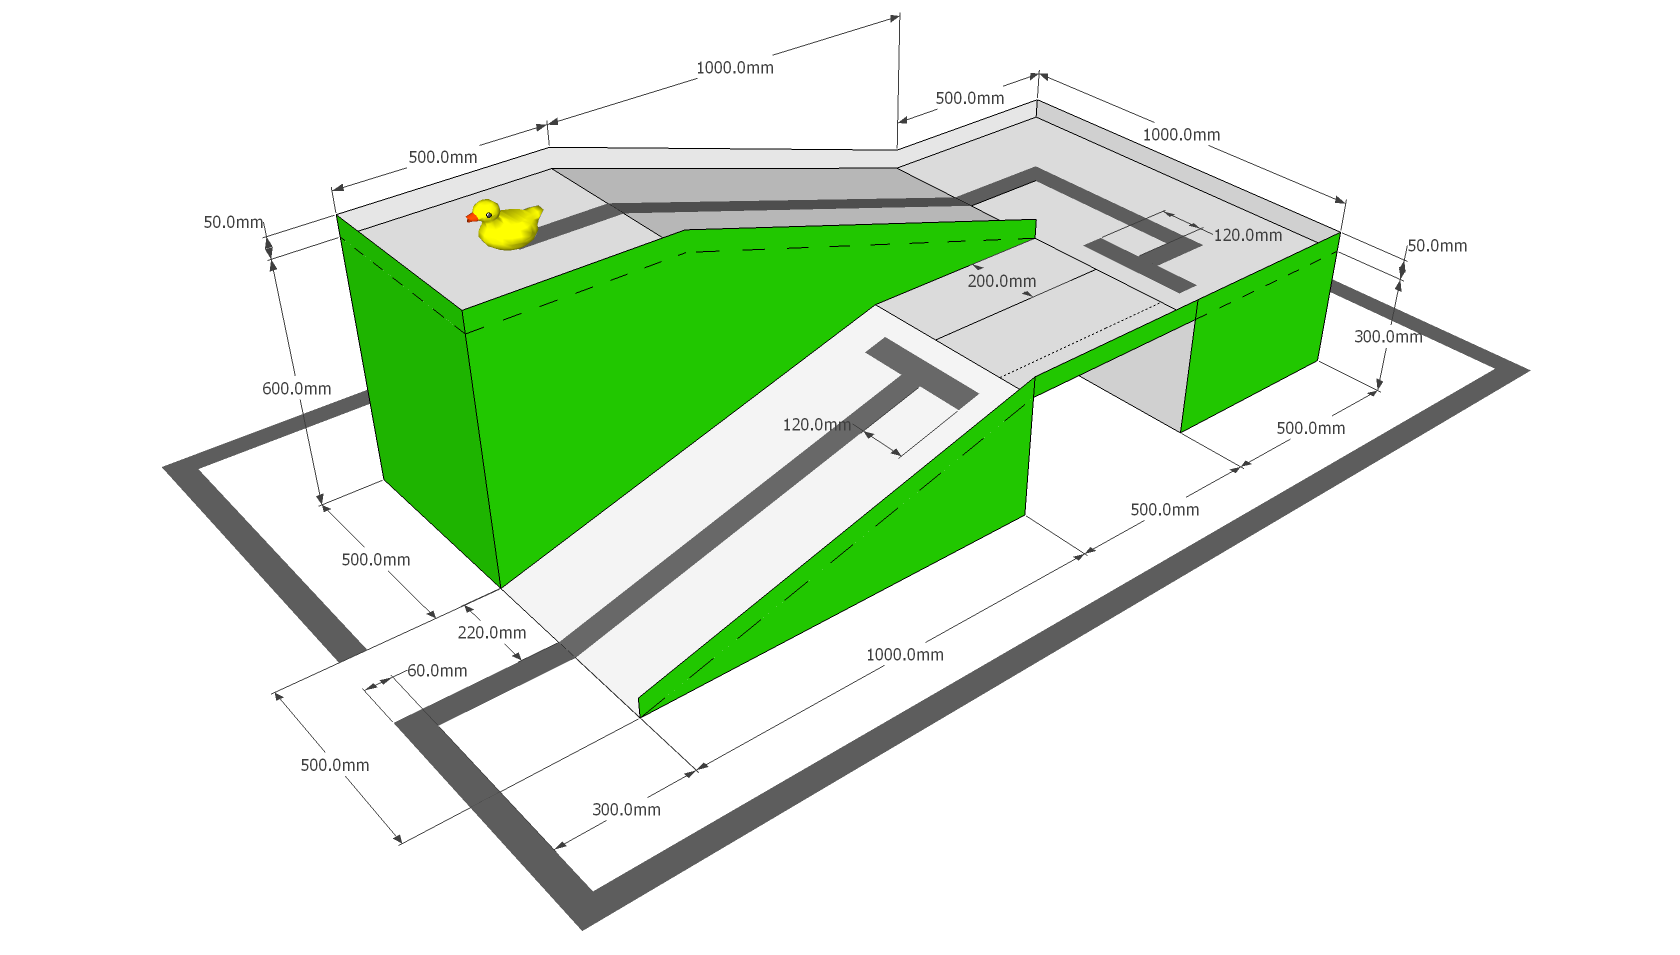
\includegraphics[keepaspectratio, trim=2cm 0 1cm 0, clip, width=\textwidth]{./images/SR2010-Ramp.png}
  \caption{\label{fig:ramp-dim}Ramp shape and dimensions.  All dimensions are in millimetres.  The line on the floor is shown in light grey for clarity, but in reality it will actually be black.  The dashed lines show the level of the ramp floor through the safety barrier, and are not present on the real, physical ramp.}
\end{figure}

\begin{figure}
  \begin{center}
    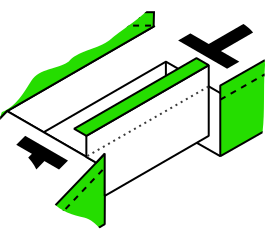
\includegraphics[keepaspectratio,width=0.4\textwidth]{./images/trapdoor-start.pdf}
  \end{center}
  \caption{\label{fig:trapdoor-open}The trapdoor in its initial, open state.  The dotted line across the trapdoor shows the line about which the trapdoor pivots.}
\end{figure}

\subsection{Tokens}
\label{tokens}
\begin {enumerate} 
\item Tokens are cubes of side $45\pm5mm$.
 Each team's kit contains a small number of these.
\item Tokens weigh $40\pm10g$.
\item A token can be either red or blue.
\end {enumerate}

\subsection{Robot Flags}
\label{sec:flags}
Robots may have a flagpole that supports the optional team flag, which
is to be designed and created by the team. The team flag allows the
robot to be easily identified.  This flag must be mounted between
$800mm$ and $1m$ off the ground.  It must not extend more than $200mm$
from the flagpole, and must not sag below $800mm$ above the ground.

The flagpole must be removable so that the robot can be placed within a box to check the size limit.
A diagram of the flagpole arrangement can be found in figure~\ref{fig:flag}.

\begin{figure}
\begin{center}
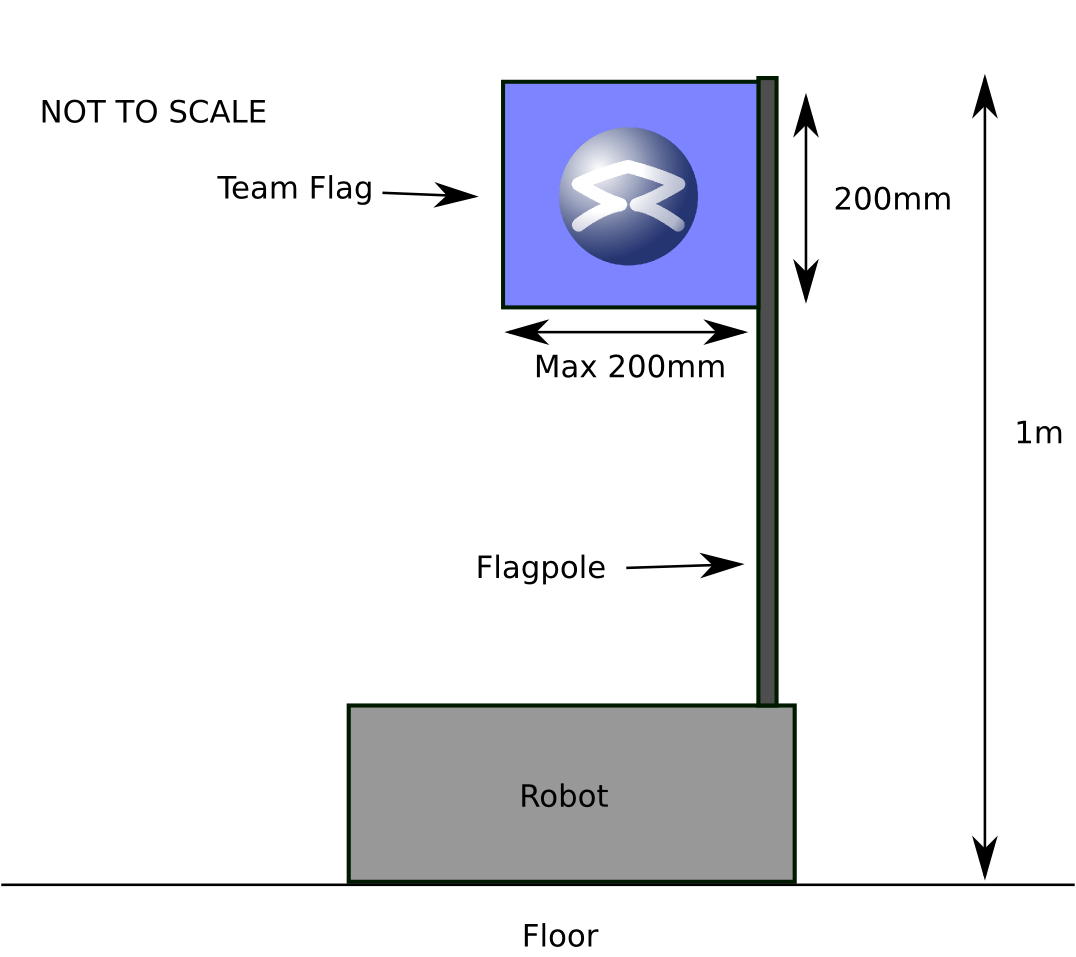
\includegraphics[keepaspectratio, scale =1]{./images/flag.png}
\caption{\label{fig:flag}Flagpole Dimensions}
\end{center}
\end{figure}
\clearpage
